\documentclass[a4paper]{article}

%% Language and font encodings
\usepackage[english]{babel}
\usepackage[utf8x]{inputenc}
\usepackage[T1]{fontenc}

%% Sets page size and margins
\usepackage{geometry}

%% Useful packages
\usepackage{amsmath}
\usepackage[table,xcdraw]{xcolor}
\usepackage{graphicx}
\usepackage{lastpage}
\usepackage[colorinlistoftodos]{todonotes}
\usepackage[colorlinks=true, allcolors=black]{hyperref}
\usepackage{fancyhdr}
\usepackage{float}

\geometry{a4paper,left=3cm, right=3cm, top=3cm, bottom=3cm}
\pagestyle{fancy}
\fancyhead[L]{Teamprojekt: SnakeKI}
\fancyhead[C]{~~~~~Snake Dokumentation Tests}
\fancyhead[R]{\today}
\fancyfoot[L]{}
\fancyfoot[C]{Seite \thepage /\pageref{LastPage}}
\fancyfoot[R]{Julia Hofmann, Marco Piechotta}
\renewcommand{\headrulewidth}{0.4pt}
\renewcommand{\footrulewidth}{0.4pt}
\parindent0pt

\begin{document}
\tableofcontents
\section{PathFindingTests}
\begin{figure}[H]
	\centering
	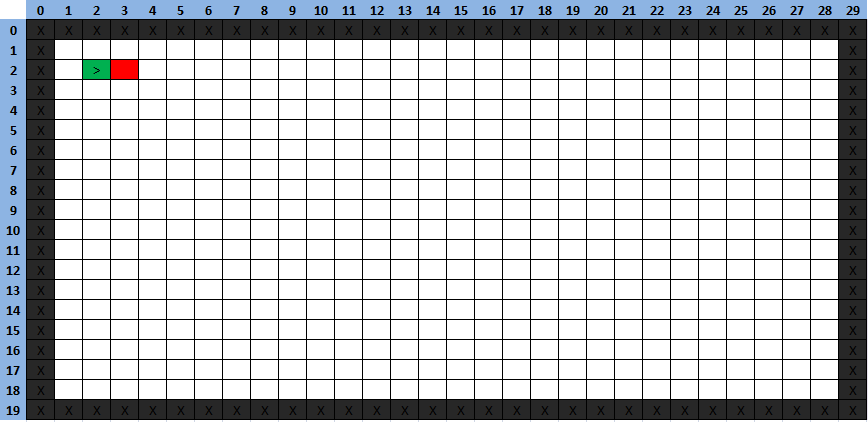
\includegraphics[width=1\textwidth]{PathfindingTest-testOneMove.png}
	\caption{testOneMove}
\end{figure}
\begin{figure}[H]
	\centering
	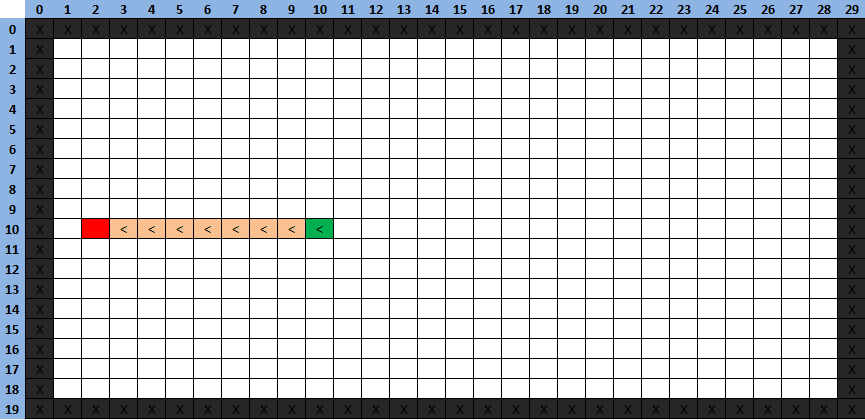
\includegraphics[width=1\textwidth]{PathfindingTest-testLeftMoves.png}
	\caption{testLeftMoves}
\end{figure}
\begin{figure}[H]
	\centering
	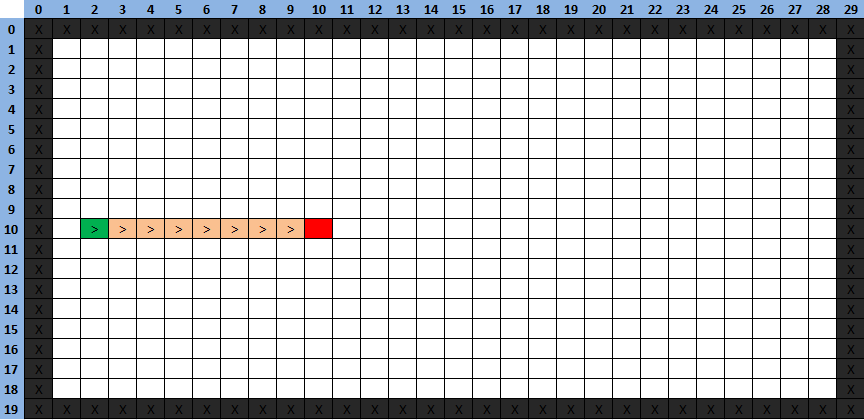
\includegraphics[width=1\textwidth]{PathfindingTest-testRightMoves.png}
	\caption{testRightMoves}
\end{figure}
\begin{figure}[H]
	\centering
	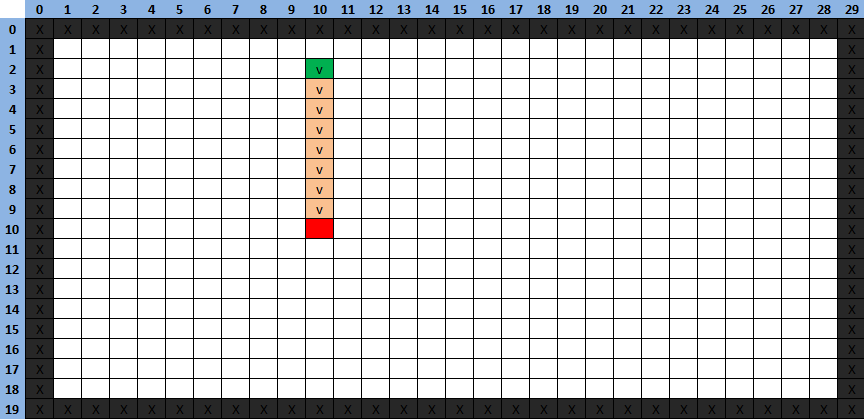
\includegraphics[width=1\textwidth]{PathfindingTest-testDownMoves.png}
	\caption{testDownMoves}
\end{figure}
\begin{figure}[H]
	\centering
	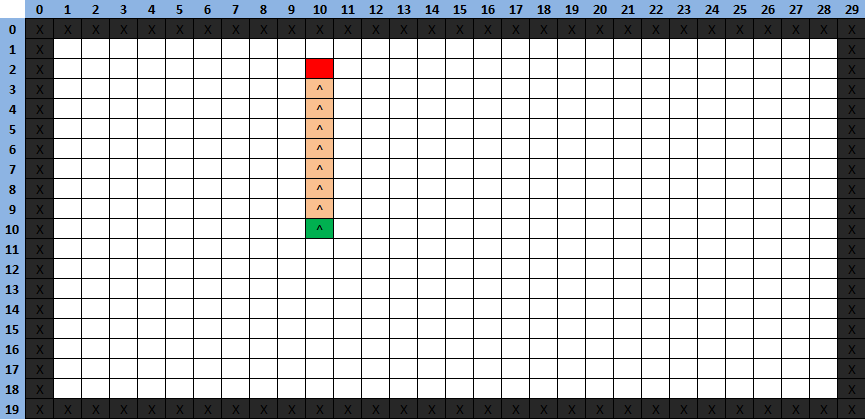
\includegraphics[width=1\textwidth]{PathfindingTest-testUpMoves.png}
	\caption{testUpMoves}
\end{figure}
\begin{figure}[H]
	\centering
	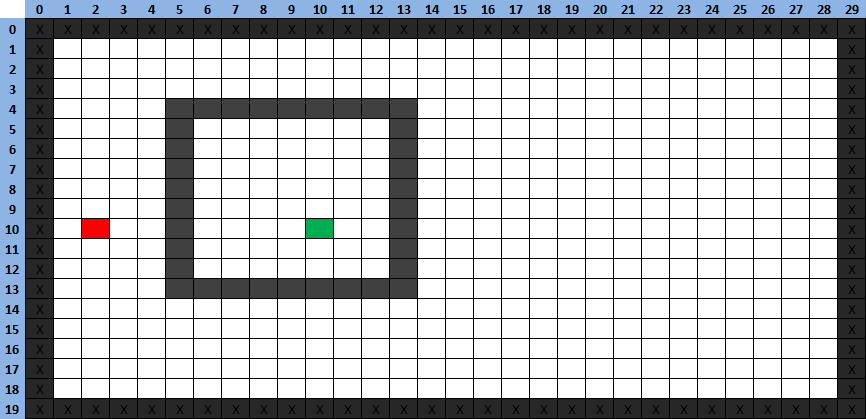
\includegraphics[width=1\textwidth]{PathfindingTest-testNoPath.png}
	\caption{testNoPath}
\end{figure}

\section{HamiltonPathTests}
\begin{figure}[H]
	\centering
	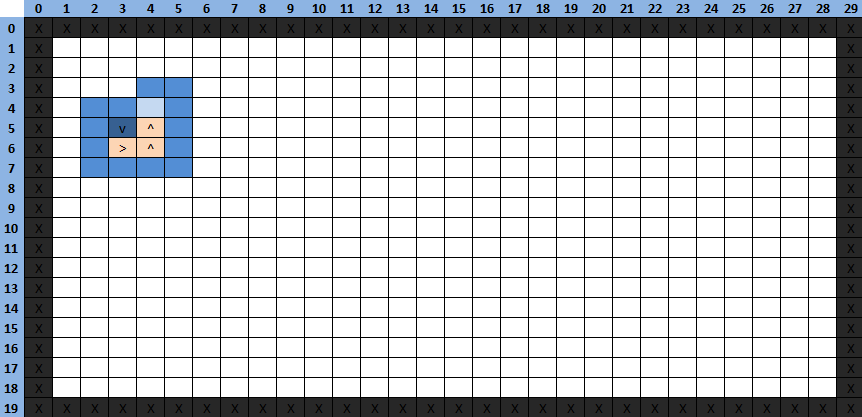
\includegraphics[width=1\textwidth]{HamiltonPathTest-testTailRightOverHead.png}
	\caption{testTailRightOverHead}
\end{figure}
\end{document}}
